\chapter{A Vision Transformer approach}\label{chapter8}
As presented in \Cref{chapter3}, vision transformers include most of the dominant models in most computer vision task.

In this section, we train a Vision Transformer model to address this problem and explore some possible ways to interpret them. The task of training a transformer was, however, not exempt from difficulties. Transformers are in general big models, which require significant resources to train.

After exploring different transformer architectures (ViT, DeiT…) we chose the MIL ViT model, a simple variation of ViT introduced by a group of Chinese researchers that we briefly commented in \Cref{chapter3} (\Cref{fig:mil_vt}). The model overcomes the dependence of ViT on a single classification token by introducing an additional multiple instance learning (MIL) classifier.

The MIL classifier creates a bag-level classification of the patches, which have been previously been reduced to a lower dimension and normalized. The resulting model is then pretrained in a large fundus image.

\begin{figure}[tb]
    \centering
    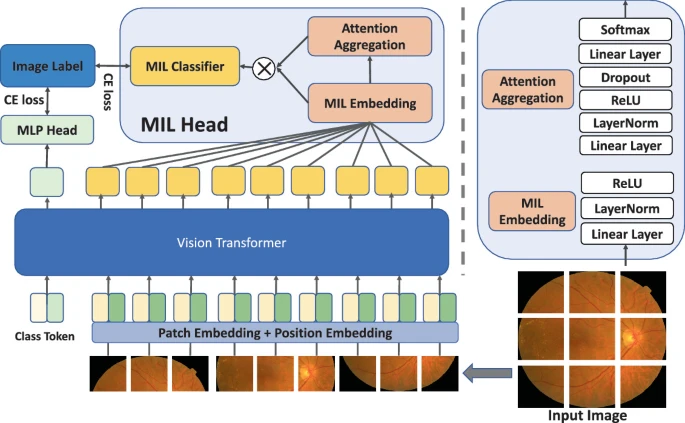
\includegraphics[width=\textwidth]{figures/chapter7/mil_vt.png}
    \caption{The restriction of ViT to a single classification token can be overcome by providing an extra MIL classifier and training both at the same time \cite{suang2021milvt}}
    \label{fig:mil_vt}
\end{figure}

This model offers an improvement over plain ViT and has the advantage of having been pretrained in a fundus dataset (not including Kaggle images), reducing the necessity of extensive finetuning. 

\section{Training a vision transformer}
In order to fine-tune the model for our case, we use the code and the weights provided by the researchers, although the code required some adaptations before we could use it on our dataset.

Even for small size images (386×386) the ViT model is too large to be fully loaded and trained in our GPU. To address this problem, we used mixed precision \cite{micikevicius2017mixed} and only retrained the classifiers (both the MIL and the standard one) and the attention layers, a technique that has proved to offer good results \cite{avidan2022things}.

Despite these measures, we found that the model required a long training time and performance was inferior to that offered by CNN. Other techniques to optimize training, like LoRA \cite{hu2021lora}, did not seem to improve the training process. 

\begin{figure}[tb]
    \centering
    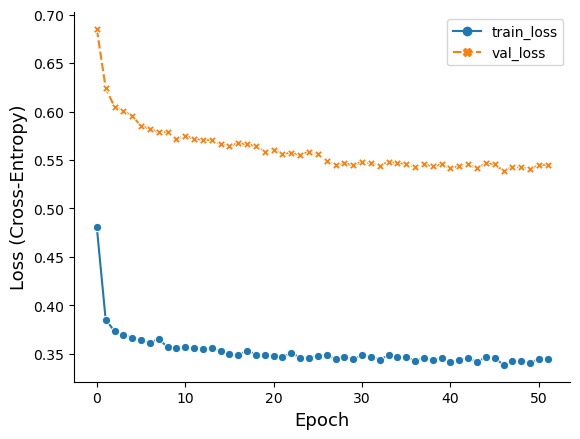
\includegraphics[scale = 0.5]{figures/chapter7/loss.png}
    \caption{Loss evolution during training.}
    \label{fig:transformer_training}
\end{figure}

We trained the transformer for 50 epochs, observing convergence to a worse optimum than CNN (\Cref{fig:transformer_training}). Following the methodology of the original authors, we used as loss function the sum of the cross-entropy loss on both classifiers.

We made several adjustments to the learning rate during the process, in order to prevent overfitting. 

At the end, we obtained a Cohen's kappa value of \( \kappa = 0.72 \). This is a reasonable result, since we are using lower resolution images (386×386 vs 512×512 for the CNN) and we are training a small fraction of the total parameters.

\section{Visualizing transformers}
One of the main advantages of using transformers is the possibility to use attention to create visualizations of the main areas of interests using a technique called \textit{attention rollout}\cite{abnar2020quantifying}.

\textit{Attention maps} do not intermix local information as CNN class activation maps do (the design of Vision Transformer does not include any concept of locality) and therefore can be used to recognize low size features\cite{dosovitskiy2020image}.

The idea behind attention rollout is simple: suppose we have two layers \( l_i, l_j \) of attention in positions \( i, j \) with \( i < j\) and two nodes \( v \in l_i \), \( u \in l_j \). We can calculate how much of the information present at \( v \) is propagated to \( u \) through a certain path by multiplying the weights of all edges in that path. If we want to calculate the total amount of information propagated, we sum over all paths between these two nodes. This is equivalent to recursively calculating \( \widetilde{A}(l_{i})\) where:
\[
\widetilde{A}(l_{i}) = \begin{cases}
A(l_i) \widetilde{A}(l_{i-1}) & \text{if \( i > j\)} \\
A(l_i)  & \text{if \( i = j\)} \\
\end{cases}
\]

In \Cref{fig:attention_comparison} we compare the class activation map for the CNN presented in \Cref{chapter5} with the attention map obtained using rollout. The attention map covers much more precisely all the lesions on the image, while the CAM is prone to artifacts. In the case of small isolated lesions the absence of other abnormalities in the patch may flatten the CAM in the region, leaving them uncovered. These properties not only make attention map superior for model explainability but also for related task like weakly supervised segmentation.

\begin{figure}[tb]
     \begin{subfigure}[b]{0.32\textwidth}
         \centering
         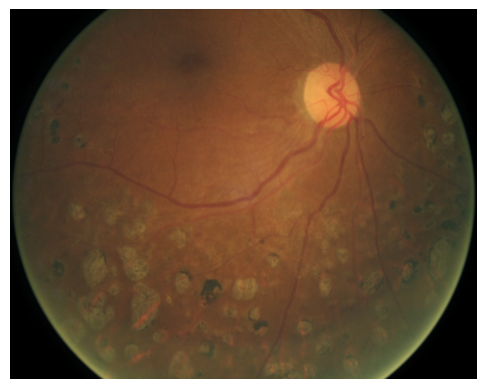
\includegraphics[width=\textwidth, height=\textwidth]{figures/chapter7/attention/43670_left_hr.png}
    \end{subfigure}
    \hfill
    \begin{subfigure}[b]{0.32\textwidth}
         \centering
         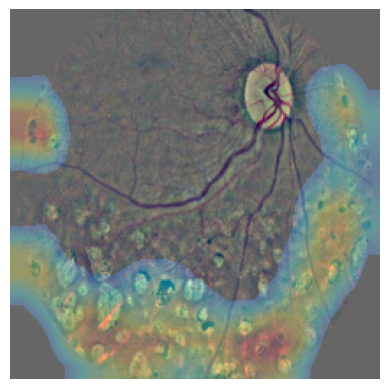
\includegraphics[width=\textwidth, height=\textwidth]{figures/chapter7/attention/43670_left_heatmap.png}
     \end{subfigure}
    \hfill
    \begin{subfigure}[b]{0.32\textwidth}
         \centering
         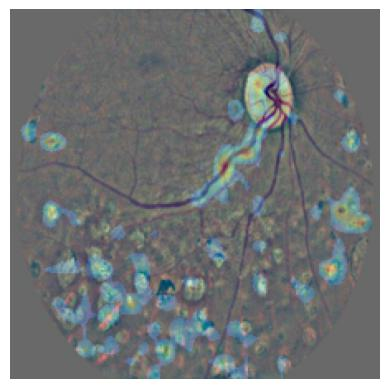
\includegraphics[width=\textwidth, height=\textwidth]{figures/chapter7/attention/43670_left_attention.jpeg}
    \end{subfigure}
    \bigskip
     \begin{subfigure}[b]{0.32\textwidth}
         \centering
         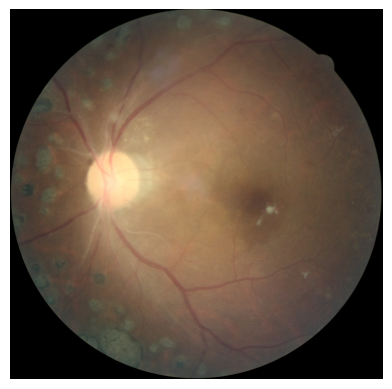
\includegraphics[width=\textwidth, height=\textwidth]{figures/chapter7/attention/28699_left_hr.png}
         \caption{Original image}
    \end{subfigure}
    \hfill
    \begin{subfigure}[b]{0.32\textwidth}
         \centering
         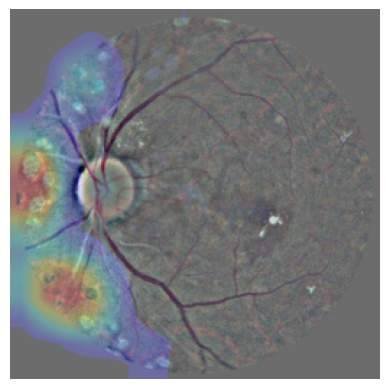
\includegraphics[width=\textwidth, height=\textwidth]{figures/chapter7/attention/28699_left_heatmap.png}
         \caption{CNN CAM}
     \end{subfigure}
    \hfill
    \begin{subfigure}[b]{0.32\textwidth}
         \centering
         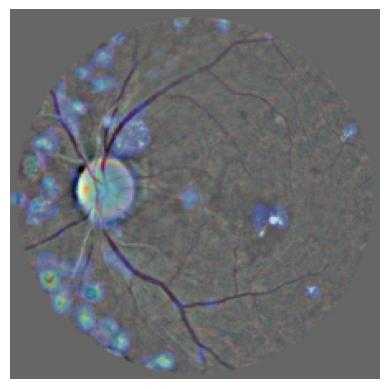
\includegraphics[width=\textwidth, height=\textwidth]{figures/chapter7/attention/28699_left_attention.jpeg}
         \caption{Attention rollout}
    \end{subfigure}
    \caption{Comparison between CNN CAM and attention map for model interpretability}
    \label{fig:attention_comparison}
\end{figure}

\section{Reflections on vision transformers}
While some authors believe vision transformers are ready to replace CNNs for most medical imaging tasks \cite{matsoukas2021time}, our experience leads  us to believe there is still significant progress to be made in the optimization of vision transformers before they can compete with CNNs in situations with restricted computational power.

The techniques used to accelerate the training of transformer-based language models and reduce its computational requirements, like quantization \cite{dettmers2022llm} or low-rank adaptation \cite{hu2021lora}, do not transfer well to vision transformers in our experience. Indeed, most techniques we used to accelerate training severely deteriorated its performance.

While more conclusive evidence is necessary, these findings endorse our initial choice of a CNN as the backbone of our model, despite its more limited interpretability properties.

